%!TEX root = main.tex

\section{Analysis of Voice Recognition Flows}

In this section, we first describe the framework that is used to analyze the factors related to user performance in voice recognition, then make use of the framework to analyze their impact, and finally summarize the results.

\subsection{Analysis Framework}

\begin{figure}[th]
\centering
	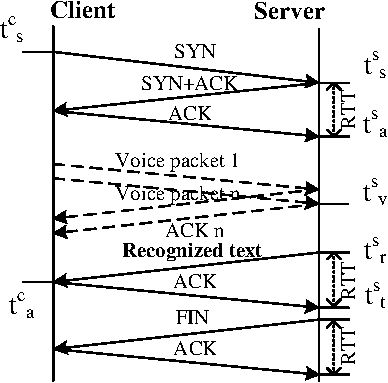
\includegraphics[scale=0.7]{voice_estimate_rtt}
\caption{Time-line in voice recognition flow.}
\label{fig:voice_estimate_rtt}
\end{figure}

Figure~\ref{fig:voice_estimate_rtt} shows the time-line in voice recognition flow. From client side, the finish time is from that client initiates the connection to that client receives all acknowledgments of the voice data, \ie $t^c_a - t^c_s$. From server side, finish time is approximated as $(t^s_t - t^s_s) - (t^s_r - t^s_v)$, where $t^s_v$ is the time that server receives all voice data, which is the duration between the time that server establishes connection and that server receives acknowledgment of the recognized text, excluding the time consumed when translating voice into text. Mainly as a receiver, server could measure at most 3 RTT's in voice recognition, which are also illustrated in Figure~\ref{fig:voice_estimate_rtt}. The three RTT's corresponds to the duration for establishing connection ($t^s_a - t^s_s$), transmitting recognized text ($t^s_t - t^s_r$), and terminating the connection.

\begin{figure*}[th]
\centering
	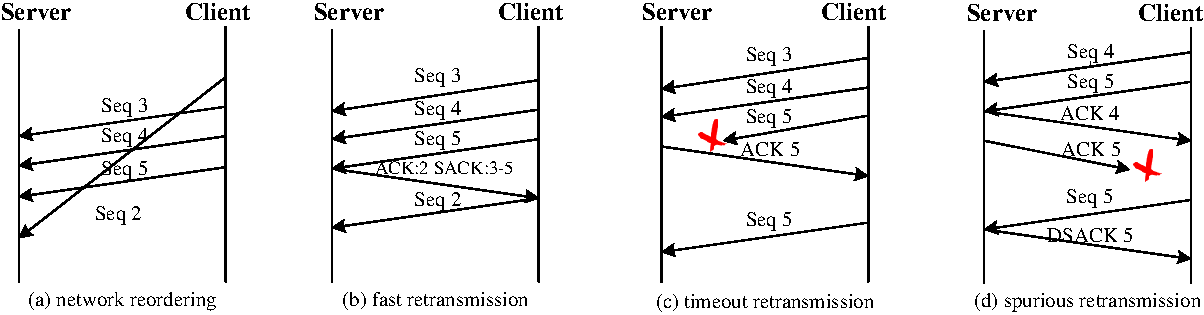
\includegraphics[scale=0.7]{voice_flow_estimate_retrans}
\caption{Server could not distinguish network congestion event when receiving voice data.}
\label{fig:voice_flow_estimate_retrans}
\end{figure*}

RTT is ambiguous when the corresponding segment is retransmitted. To investigate the impact of RTT on finish time, we use the following strategy to determine the minimal RTT. If there is no retransmission of SYN packet, $t^s_a - t^s_s$ is used as the RTT of the flow. Otherwise, the RTT when server terminates the connection is used, if the FIN packet is not retransmitted. When both of the two RTT's above are ambiguous, $t^s_t - t^s_r$ is exploited. We have verified in the web search dataset that $t^s_a - t^s_s$ is the minimal RTT in more than 60\% of flows, and is less than 2 times of the minimal RTT in 95\% of flows. Thus it is reasonable to assume that the measured RTT from server side could represent the minimal RTT from client side in voice recognition.

Besides the estimation of RTT, server could not distinguish network congestion event when receiving data from client, which is exemplified in Figure~\ref{fig:voice_flow_estimate_retrans}. In Figure~\ref{fig:voice_flow_estimate_retrans}(a), there are packets reordered by network, which has the same appearance at server side as that with fast retransmission in Figure~\ref{fig:voice_flow_estimate_retrans}(b). Actually, there is no packet loss in the former case, while there is in the latter case. In Figure~\ref{fig:voice_flow_estimate_retrans}(c), client retransmitted segment 5 when RTO timer is triggered. Server could not detect that the packet is retransmitted or reordered, but only sense that the packet is delayed for a longer time, compared to other packets. In fact, server could only detect unnecessary retransmission when receiving the same data packet twice, and notifies the spurious retransmission to client via Duplicate SACK~\cite{rfc3078}, which is shown in Figure~\ref{fig:voice_flow_estimate_retrans}(d).

To depict network congestion, we need two more metrics besides RTT: packet reordering and timeout retransmission. We use the number of disordered packets to represent the severity of packet reordering, which is defined as follows. In receiving sequence $S_1, S_3, S_4, S_2$, the packet $S_2$ is disordered, thus the number of disordered packets is 1. In the following, we will take packet reordering as an indication of network congestion and study the impact of network reordering on finish time.

Timeout retransmission corresponds to more severe network congestion. As illustrated in the figure above, timeout retransmission could not be directly identified by server when receiving voice data. We rely on the following estimation to detect timeout retransmission. In TCP/IP stack, RTO timer is set to SRTT + max(200ms, 4 RTTVAR)\cite{rfc62982011computing}, where SRTT is approximated to RTT, and RTTVAR is approximated to RTT/2. Thus RTO could be represented as RTT + max(200ms, 2 RTT). For each packet, there is an estimated arrival time, calculated according to that of preceding and subsequent packets. If the gap between actual arrival time and the estimated arrival time is larger than RTT + max(200ms, 2 RTT), it is identified as a RTO. In the following, we also investigate the impact of timeout retransmission on finish time in voice recognition.

\subsection{Analyzing the impact on Finish Time}

In this section, we first show the poor performance that voice recognition flows experience, which inspires us to understand how the network condition leads to such results.

\begin{table}[th]
\centering
\renewcommand{\arraystretch}{1.2}
\caption{Percentage of flows with timeout retransmission in different access types.}
\label{tab:voice_stats}
\begin{tabular}{l|c|c|c}
	\toprule
	 & WiFi & 2G & 3G \\
	\midrule
	% packet reordering & 3.2\% & 5.6\% & 6.2\% \\
	% \hline
	SYN retransmission & 2.6\% & 1.4\% & 0.8\% \\
	\hline
	data timeout retransmission & 9.5\% & 8.0\% & 7.3\% \\
	% \hline
	% incomplete transmission & 0.2\% & 0.3\% & 2.4\% \\
	\bottomrule
\end{tabular}
\end{table}

Table~\ref{tab:voice_stats} shows the percentage of flows with timeout retransmission in each access type. The timeout retransmission could happen during 3-way handshake, or in data transmission.

In the table, about $0.8\% \sim 2.6\%$ of flows encounter RTO when establishing connections, which is named SYN retransmission. Flows in WiFi network are more likely to experience SYN retransmission than those in 2G/3G network. SYN retransmission greatly harms the finish time due to two reasons. First, the time for establishing connections is irrelevant to data transmission, yet occupies huge portion of flow latency. Second, the initial RTO is set to 1 second \cite{rfc62982011computing} as there is no RTT measured. When the SYN packet is dropped, it has to wait at least 1 second for retransmission, which is another great penalty to the finish time.

About $7.3\% \sim 9.5\%$ of flows experience timeout retransmission when transferring data packets. Also flows in WiFi network are more likely to have timeout retransmission than those in 2G/3G network. However, the disparity of flows with data timeout retransmission among different access types is not that large, compared to SYN retransmission. In voice recognition flows, timeout retransmission has a devastating effect on the performance, and is easy to be activated. Most of voice recognition flows have no more than 6 data packets. When one of the last three packets is dropped, sender has to rely on RTO for retransmission. Compared to the ideal data transmission time, RTO is often tens of, or even hundreds of times higher \cite{flach2013reducing}.

% Table~\ref{tab:voice_stats} also shows the percentage of incomplete flows. An extreme case is that the percentage of incomplete flows is 2.4\% in CM. The flow is terminated before finishing data transmission, either by TCP stack after several RTO's, or by consumer after waiting for an intolerably long time. The non-negligible ratio of incomplete flows indicates poor user-perceived performance, which motivates us to understand the reasons behind.

\begin{table}[th]
\caption{The average RTT value and number of disordered packets in different access types.}
\label{tab:voice_access_type_stats}
\centering
\renewcommand{\arraystretch}{1.2}
\begin{tabular}{l|l|l|l}
	\toprule
	& WiFi & 2G & 3G \\
	\midrule
	RTT (s) & 0.119 & 0.067 & 0.054 \\
	\hline
	\#(disordered packets) & 0.012 & 0.019 & 0.020 \\
	\bottomrule
\end{tabular}
\end{table}

Table~\ref{tab:voice_access_type_stats} shows the average RTT and number of disordered packets of each flow for different access types. From the table, we could see that flows in different access types experience different network conditions. For example, compared to flows in cellular network (2G/3G), the flows in WiFi network have larger RTT values, yet fewer disordered packets. The average RTT value in WiFi network is one time larger than that in 2G/3G network; however, the average number of disordered packets in WiFi is nearly one half of that in 2G/3G network.

\begin{figure}[th]
	\centering
	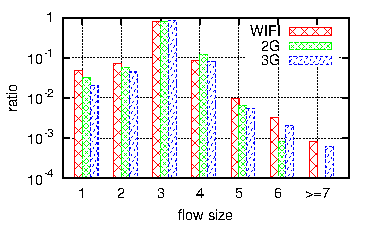
\includegraphics[width=0.8\linewidth]{voice_flow_size}
	\caption{The distribution of flow sizes in voice recognition.}
	\label{fig:voice_flow_size}
\end{figure}

First, we study the impact of flow size on finish time in voice recognition. The distribution of flow sizes are shown in Figure~\ref{fig:voice_flow_size}, in which the $y$-axis is drawn in log scale.. Note that flow size does not include the packet carrying text in voice recognition. From the figure, nearly all flows contain no more than 6 data packets. Among all access types, about 80\% of voice recognition flows are with 3 data packets. The initial congestion window in current Android TCP/IP stack is set to 10 segments\cite{dukkipati2010argument}, which means the voice data could be transmitted in the initial congestion window.

We use Kendall correlation coefficient to inspect their relationship in the three access types. The absolute values of the coefficients are less than 0.003, which demonstrates that the finish time is completely irrelevant to the flow size. As the voice data in most of flows could be packed within the initial congestion window from client side. Thus ideally finish time is 2 times the RTT value, one for establishing connection, and one for transmitting data.

\begin{figure}[th]
\centering
	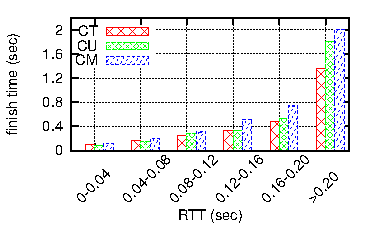
\includegraphics[width=0.8\linewidth]{voice_rtt}
\caption{The distribution of RTT's in voice recognition flows.}
\label{fig:voice_rtt}
\end{figure}

Next, we study the impact of RTT on the finish time in voice recognition. Figure~\ref{fig:voice_rtt} shows the CDF of RTT's in voice recognition. From the figure, cellular network (with median RTT value 0.033s) presents smaller RTT's than WiFi network (with median RTT value 0.049s). About 95\% of flows in cellular network have RTT smaller than 0.1s, while 20\% of flows in WiFi network have RTT larger than 0.1s. The different distributions of RTT's in different access types make us to investigate the impact of RTT separately.

\begin{table}[th]
\caption{Finish time under different RTT values in cellular network using QED.}
\label{tab:voice_celluar_qed_rtt}
\centering
\renewcommand{\arraystretch}{1.2}
\begin{tabular}{l|m{.35in}|m{.35in}}
	\toprule
	RTT bin (s) & 2G & 3G \\
	\midrule
	$[$ 0.01, 0.02 ) & 5.12 & 3.71 \\
	\hline
	$[$ 0.02, 0.03 ) & 6.20 & 5.06 \\
	\hline 
	$[$ 0.03, 0.04 ) & 9.94 & 10.84 \\
	\hline 
	$[$ 0.04, 0.05 ) & 9.56 & 11.44 \\
	\hline 
	$[$ 0.05, 0.06 ) & 13.73 & 15.18 \\
	\hline 
	$[$ 0.06, 0.07 ) & 16.74 & 16.74 \\
	\hline 
	$[$ 0.07, 0.08 ) & 23.50 & 18.95 \\
	\hline 
	$[$ 0.08, $\infty$ ) & 106.41 & 62.30 \\
	\bottomrule
\end{tabular}
\end{table}

In cellular network, there are less than 5\% of flows with RTT larger than 0.08s. Thus in the QED experiment, we use 0.01s interval to group the flows into 9 bins by their RTT's, and take the flows in the RTT bin $[$0, 0.01) as the baseline. For each flow in this bin, we randomly choose a flow in each of other bins, which has the same access type, equal number of disordered packets, and the same condition whether encountering timeout retransmission. The results are shown in Table~\ref{tab:voice_celluar_qed_rtt}. In the table, when the RTT value is no more than 0.08s, finish time is approximately proportional to the RTT value, which verifies our assertion above. Furthermore, when RTT value is larger than 0.08s, the finish time become incredibly large (106 times the baseline value). This could be explained as follows. Larger RTT indicates that the packets are buffered in the network for longer time, which is also a signal of network congestion, as used in TCP Vegas\cite{brakmo1995tcp} and FastTCP\cite{wei2006fast}. Thus when flow experiences large RTT, it is likely that the flow is traversing congested network, and may encounter packet loss, takes at least one RTT (or even RTO) for recovery.

\begin{table}[th]
\caption{Finish time under different RTT values in WiFi network using QED.}
\label{tab:voice_wifi_qed_rtt}
\centering
\renewcommand{\arraystretch}{1.2}
\begin{tabular}{l|l}
	\toprule
	RTT bin (s) & WiFi \\
	\midrule
	$[$ 0.04, 0.08 ) & 5.78 \\
	\hline
	$[$ 0.08, 0.12 ) & 10.13 \\
	\hline
	$[$ 0.12, 0.16 ) & 15.46 \\
	\hline
	$[$ 0.16, 0.20 ) & 20.17 \\
	\hline
	$[$ 0.20, $\infty$ ) & 70.83 \\
	\bottomrule
\end{tabular}
\end{table}

For WiFi data, we use 0.04s interval and takes the flows in the RTT bin $[$0, 0.04) as the baseline, the strategy to choose flows is the same as above. The QED result is shown in Table~\ref{tab:voice_wifi_qed_rtt}. Similarly, the finish time is proportional to the RTT value, except last RTT bin. When RTT is larger than 0.2s, finish time becomes 70 times the baseline value.

\begin{figure}[th]
\centering
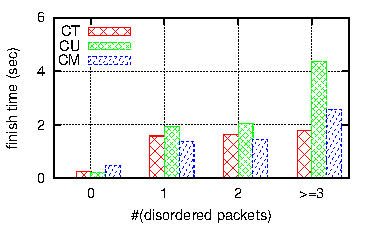
\includegraphics[width=3in]{voice_reorder}
\caption{The finish time under different number of disordered packets in voice recognition.}
\label{fig:voice_reorder}
\end{figure}

RTT affects finish time by increasing the time to acknowledge received data, while packet reordering affects finish time by increasing the number of rounds for data transmission. To study the impact of packet reordering, we first show the distribution of packet reordering in Table~\ref{tab:voice_reorder}.

\begin{table}[th]
\caption{Distribution of flows with different packet reordering in voice recognition.}
\label{tab:voice_reorder}
\centering
\renewcommand{\arraystretch}{1.2}
\begin{tabular}{c|c|c|c}
\toprule
\#(disordered packets) & WiFi & 2G & 3G \\
\midrule
0 & 96.7\% & 94.4\% & 93.3\% \\
\hline
1 & 3.03\% & 5.5\% & 6.6\% \\
\hline
2 & 0.1\% & - & - \\
\hline
$\ge$3 & 0.1\% & - & - \\
\bottomrule
\end{tabular}
\end{table}

In the table, most of flows do not have disordered packet. Flows in WiFi network and cellular network experience different types of packet reordering. In WiFi network, the ratio of flows with disordered packets is small, while there are flows with 3 or more disordered packets. Even though cellular network have more disordered packets, there are hardly flows with 2 or more disordered packets.

\begin{table}[th]
\caption{Finish time under different number of disordered packets.}
\label{tab:voice_qed_reorder}
\centering
\renewcommand{\arraystretch}{1.2}
\begin{tabular}{c|c|c|c}
	\toprule
	\#(disordered packets) & WiFi & 2G & 3G \\
	\midrule
	1 & 7.42 & 4.37 & 5.45 \\
	\hline
	2 & 10.4 & - & - \\
	\hline
	$\ge$3 & 11.8 & - & - \\
	\bottomrule
\end{tabular}
\end{table}

Table~\ref{tab:voice_qed_reorder} presents the QED results showing the impact of packet reordering on finish time. In the experiment, we group the flows into bins by counting the number of disordered packets, and take the flows with no disordered packet as baseline. For each flow in the baseline, we randomly choose a flow from each of other bins, which has similar RTT value (using 0.04s interval), the same access type, and the same condition whether encountering timeout retransmission. From the table, as there are nearly no flow with 2 or more disordered packets in cellular network, the corresponding values are not calculated. When there is only one disordered packet, the finish time is 3-6 times higher than the baseline value. \textbf{How to explain this?}

% Figure~\ref{fig:voice_reorder} shows the average finish time under different number of disordered packets. In cellular network, there are quite few flows with more than 1 disordered packet. Thus the corresponding bins are left blank. From the figure, in all networks, when there are disordered packets, flows experience significant performance degradation. Even when there is only 1 disordered packet, the average finish time is 2$\sim$3 times higher than that of flows without disordered packet. This could be explained as follows. If server receives packets which are not successive, it feeds back to the client with SACK. When receiving SACK, client does not retransmit the packet in the hole (\ie the disordered packet) immediately, until client receives 3 SACK's or ACK of that packet, or retransmission timer is triggered. If the packet is dropped, client needs to wait at least one RTT to retransmit the packet. If there are no sufficient number of SACK's, client has to rely on timeout retransmission (RTO). The RTO timer, as an estimate of RTT and its variation, is usually highly conservative, which is set to tens of, or even hundreds of RTT.

\begin{figure}[th]
\centering
	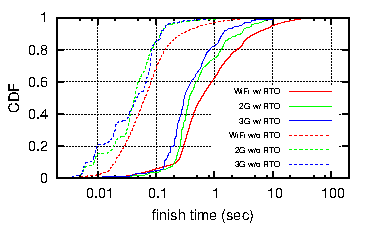
\includegraphics[width=\linewidth]{voice_timeout}
\caption{CDF of finish time of flows with and without RTO.}
\label{fig:voice_rto}
\end{figure}

Figure~\ref{fig:voice_rto} shows the CDF of finish time of flows with and without RTO. Note that the x-axis in the figure is plotted in log scale. From the figure, there is a remarkable performance gap between flows with RTO and that without RTO. The gap could be ten times as for the median values. If there is no RTO, client needs 2-7 RTT's to transmit the voice data (1 RTT for each packet in worst case). However, if a packet is dropped and there are no sufficient subsequent data packets, the RTO will occupy most of the finish time. Among the flows with timeout retransmission, more than 50\% of flows are with ratio RTO/RTT larger than 10, 10\% of flows are with ratio larger than 100.

\subsection{Summary of Voice Recognition Analysis}

The key observations on voice recognition flows are summarized as follows.
\begin{itemize}
	\item Almost all voice recognition flows contain less than 7 data packets, which could be fitted into the initial congestion window from Android client. Thus ideally the voice data could be transmitted in 1 RTT.
	\item Finish time is affected by RTT. For flows with smaller RTT (less than 200ms in WiFi), the finish time is proportional to the RTT value. However, flows with larger RTT experience intolerably long finish time, caused by timeout retransmission.
	\item Flows in WiFi network experience 2-3 times longer finish time than those in cellular network, because of larger RTT.
	\item About 10\% of flows experience timeout retransmission when transmitting data, which make the finish time one order of magnitude larger than those without timeout retransmission.
	\item A non-negligible fraction of flows (0.8\%-2.6\%) experience retransmission when establishing connections, which has similar impact like RTO in data transfer.
\end{itemize}